\documentclass{article}
\usepackage[margin=1in]{geometry}
\usepackage{amsmath,amsthm,amssymb}
\usepackage{bbm,enumerate,mathtools}
\usepackage{tikz,pgfplots}
\usepackage{chessboard}
\usepackage[hidelinks]{hyperref}
\usepackage{multicol} % Problem 35

\newenvironment{question}{\begin{trivlist}\item[\textbf{Question.}]}{\end{trivlist}}
\newenvironment{note}{\begin{trivlist}\item[\textbf{Note.}]}{\end{trivlist}}
\newenvironment{references}{\begin{trivlist}\item[\textbf{References.}]}{\end{trivlist}}
\newenvironment{related}{\begin{trivlist}\item[\textbf{Related.}]\end{trivlist}\begin{enumerate}}{\end{enumerate}}


\begin{document}
\rating{3}{2}
Consider ways to partition the $n \times m$ grid so that no three tiles of the
same partition fall on a line.
\begin{figure}[!h]
  \centering
  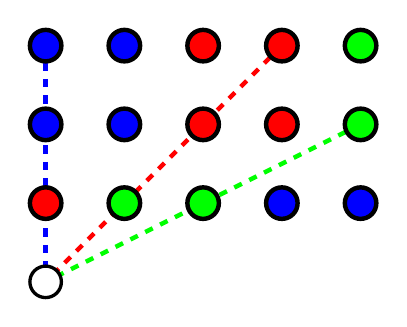
\begin{tikzpicture}
    \draw[ultra thick, blue, dashed] (0,2)--(0,-1);
    \draw[ultra thick, red, dashed] (3,2)--(0,-1);
    \draw[ultra thick, green, dashed] (4,1)--(0,-1);
    \foreach \x/\y in {0/2,1/2,0/1,1/1,3/0,4/0} { \draw[ultra thick, fill=blue] (\x,\y) circle (0.2cm); }
    \foreach \x/\y in {2/2,3/2,2/1,3/1,0/0} { \draw[ultra thick, fill=red] (\x,\y) circle (0.2cm); }
    \foreach \x/\y in {4/2,4/1,1/0,2/0} { \draw[ultra thick, fill=green] (\x,\y) circle (0.2cm); }
    \draw[very thick, fill=white] (0,-1) circle (0.2cm);
  \end{tikzpicture}
  \caption{
    A $3$ partition of the $5 \times 3$ grid. The white circle cannot be in
    any of the existing partitions, otherwise three circles of the same
    color would fall on the same line.
  }
\end{figure}

\begin{question}
  How many colors are required to satisfy the ``no three in a row'' criterion?
\end{question}
\begin{related}
  \item What if this is generalized to $k$ in a row?
  \item What if this is generalized to a triangular or hexagonal grid?
  \item What if this is generalized to a torus or cylinder or M\"obius strip?
  \item What if this only queen moves or rook moves are considered?
  \item How many distinct configurations exist with a minimal number of partitions?
  \item How many distinct configurations exist with $k$ partitions?
\end{related}
\begin{references}
  \item Problem 26.
\end{references}

\end{document}
